\documentclass[report]{BetterDocument}

\newcommand{\bdd}{base de données}

\addtocontents{toc}{\setcounter{tocdepth}{1}}

\title{Équida}
\subtitle{Doc Technique}
\who{MARTIN Justine\\
	BOTTON Léa}
\date{2019}
\place{BTS SIO 2 - Jean Rostand Caen - E4}

\graphicspath{
    {include/appli_mobile/}
    {include/appli_web/}
    {include/contexte/}
    {include/core/}
}

\begin{document}

	\pageDeGarde

	\tableDesMatieres

	\chapter{Contexte et présentation}
	\section{Présentation du contexte}
	%TODO Léa : Parler du client et de son métier + besoin (cf : Cahier des charges.pdf)
		Créée en 2006, Equida est une société spécialisée dans la vente aux enchères de chevaux de course. Avec un effectif de vingt-sept personnes, la société a réalisé en 2012 un chiffre d’affaires de 87 millions d’euros. Ses clients sont des vendeurs de chevaux, principalement des haras, des entraîneurs et de grands propriétaires de chevaux, situés en France et à l’étranger. Pour être plus proche de sa clientèle étrangère, elle s’appuie sur une quinzaine de correspondants répartis dans de nombreux pays comme l’Irlande, la Turquie, ou encore le Japon.\newline
		Pour gérer son activité, la société utilise un site web qui permet notamment la consultation des ventes, une application Planning qui permet de gérer les clients, une application de gestion desventes aux enchères ainsi qu'une application de gestion des informations des chevaux.\newline
		Equida souhaite combiner ses différentes applications en une seule qui lui permettra donc de gérer les chevaux et leurs informations, leurs mises en vente, leurs enchères ainsi qu'une gestion des clients et de leur compte. Cette application combinant des fonctionnalités pour les clients (enregistrement d'un cheval, proposition d'un cheval à une vente,...) et des fonctionnalités pour l'administrateur (gestion des clients et de leur compte, validation des propositions, ajout de ventes...), elle devra contenir deux niveaux d'authentification.
		Pour plus d'informations, vous pouvez consulter la totalité du cahier des charges : \url{https://github.com/justine-martin-study/Equida/blob/master/doc/Cahier%20des%20charges.pdf}

		\noindent
		On a fait le choix de réaliser un seul projet contenant deux applications : une application web (cf: lien vers appli web) et une application mobile (cf: lien vers appli mobile) qui utilisera une api. L'application web est plus complète car destinée à être utiliser surtout par l'administrateur ; l'application mobile, elle, se concentre surtout sur des fonctionnalités propre à l'utilisateur avec tout de même quelques possibilités de gestion pour l'administrateur.

	\section{Choix techno}

		%TODO Léa : Disclamer : Pas tuto SpringBoot, gradle, ionic, ... (mettre des liens tutos)

		\subsection{MySql}
		%TODO Léa : Pourquoi avoir choisi MySql et pas autre chose
			MySql, en comparaison avec Oracle, est open source et gratuit. Ce qui le rend avantageux. \newline
			De plus, le cahier des charges fourni par le client retenait la solution de MySql pour la base de données.

		\subsection{Spring Boot}
		%TODO Léa : Pourquoi Spring boot, parler des ""parts du marchés"", avantages, ...
			On fait le choix de SpringBoot pour le projet car c'est très probablement le Framework Java pour le développement web le plus utilisé. Il permet de créer facilement un contrôleur, en effet, il suffit de créer une classe et de l’annoter @Controller. Chacune des méthodes aura l’annotation @GetMapping, @PostMapping ou tout autre méthode HTTP ayant le modèle suivant @XMapping, qui indique l'url de la page, ainsi que sa méthode HTTP, qui lui correspond.\newline
			De plus, il embarque l'équivalent d'un serveur TomCat lors de la compilation du projet (en faisant Tasks > boot > bootRun sur netbeans ou gradle bootRun en ligne de commande) qui permet le démarrage du projet par l'intermédiaire du serveur web embarqué. \newline
			Vous pouvez retrouver ce framework ici : \url{https://spring.io/projects/spring-boot} ainsi que des tutoriels pour l'utiliser ici \url{https://www.tutorialspoint.com/spring_boot/index.htm} et là \url{https://www.javatpoint.com/spring-boot-tutorial}

		\subsection{Ionic}
		%TODO Léa : Pourquoi Ionic, écrire du code en code Js, multiplateforme, ...
			Ionic est un framework open source qui permet de créer des applications multiplateformes (mobile et navigateur) performantes tout en utilisant des technologies Web connues (HTML, CSS, JavaScript). Il possède en plus une intégration d'Angular qui permet d'appréhender une page web comme un assemblage de composants webs indépendants mais qui peuvent communiquer entre eux. \newline
			Ionic intègre également des composants visuels natifs, ainsi, les utilisateurs d'Android ou d'iOs conserveront leurs habitudes sur l'application. \newline
			Vous pouvez retrouver ce framework ici : \url{https://ionicframework.com/docs/installation/cli} avec sa documentation : \url{https://ionicframework.com/docs/components}.

		\subsection{Gradle}
			%On fait une description brève car on en reparle plus en détail dans "Intéraction entre les différentes parties du projet"
			Gradle est un "build automation system" (moteur de production). Il est un équivalent plus récent et complet à Maven. Il possède de meilleure performances, possède un bon support dans de nombreux IDE et permet d'utiliser de nombreux dépots, dont ceux de Maven.

	\section{Organisation du projet}
		\subsection{Git et branches}
			On utilise donc Git comme logiciel de gestion de versions ce qui nous permet de travailler en parallèle sur les mêmes fichiers et d'effectuer chacunes les modifications qui nous concernent sans gêner le travail de l'autre.
			\subsubsection{Branches}
			%TODO Léa : Parler de master (=version prod), develop, features/XXX
				Afin d'utiliser au mieux Git, nous avons fait le choix de créer deux branches "principales". Il s'agit donc de master et de develop.
				La branche master correspond à la version en production de nos applications. Ainsi, on ne travaillera jamais sur cette branche. Elle ne nous servira donc qu'à récupérer l'application dans un état stable afin d'y mettre les différentes applications en production.
				La branche develop, quant à elle, est donc la branche à partir de laquelle nous travaillons. C'est à partir de cette dernière que nous créons les différentes branches pour le développement de nos fonctionnalités. Ne sont poussées sur celle-ci que les nouvelles fonctionnalités opérationnels des applications. C'est donc la version en cours de développement.
				Les branches créées à partir de develop sont donc les branches correspondant aux fonctionnalités développées, elles commencent toutes par features/XXX (correspondant à la modification). Par exemple, pour la gestion des clients, on crera une branche features/gestionClients.

			\subsubsection{Nomenclature}
			%TODO Léa : Parler des nommenclatures (cf : fichier CONVENTIONS.md)
				Pour une meilleure homogénéisation de la gestion des versions, on choisit d'établir et d'utiliser une nomenclature pour les messages de commit. Cette nomenclature est consultable dans le fichier CONVENTIONS.md.
				On retrouve notamment les commits pour l'ajout de fonctionnalités sous le nom de "feat", pour les corrections de bug "fix", pour la documentation "doc", ...
				Ce qui donne des messages comme celui-ci : "feat : Ajout de la modification d'un client".


		\subsection{Les différents dossiers}
			\subsubsection{Doc}
			%TODO Léa : ((Parler de pk latex? = opensource, meilleure gestion sur git, compilation directe en pdf, ...)) + autres doc
				On a fait le choix de rédiger la documentation du projet avec Latex car c'est un système de création de documents opensource. De plus, les fichiers Latex sont facilement gérés par Git contrairement aux fichiers Word. On peut ainsi gérer aisément les différentes versions des documents. Il permet également une compilation directe au format pdf.

			\subsubsection{SQL}
			%TODO Léa : Expliquer + nommenclature et table de version
				Les fichiers SQL (situés dans le dossier /sql) sont donc ceux qui vont créer la base de données. Il suffit d'importer les scripts dans l'ordre afin de la restituer. On nomme les fichiers précédés d'un numéro (ordre d'importation) suivi de l'intitulité de la modification. Les tables de la BDD sont en majuscules séparés par des underscore si besoin tandis que les champs de plusieurs mots sont séparés par des majuscules (comme en CamelCase).

			\subsubsection{Sources}
			%TODO Léa : Ionic = ionic, spring = code spring boot(webapp, rest, core) (on en reparlera plus tard dans la doc)
				Dans le dossier source, on retrouve donc deux sous-dossiers : un sous-dossier ionic et un Spring.
				Le sous-dossier ionic, comme son nom le suggère, correspond au code prore à l'application mobile (développée avec Ionic). On retrouvera donc à l'intérieur, des fichiers json, html, service.ts. On reviendra plus en détail sur cette partie : cf lien vers le bon truc. 	%TODO Léa : FAIRE LE LIEN POV' DEBILE
				Le sous-dossier Spring, correpondant à SpringBoot, contient, quant à lui, les dossiers core, gradle, rest et webApp. Contenant notamment et respectivement les fichiers communs aux deux applications (bdd, service...), les fichiers de configuration, le code de l'api ainsi que le code de l'application web (controller, routes, formulaires, ...).
				De même, vous trouverez plus d'informations : cf lien vers le bon truc. %TODO Léa : FAIRE LE LIEN POV' DEBILE

		\subsection{Trello}
		%TODO Léa : Fournir le lien et expliquer étiquettes, Listes
			Le planning, la répartition des tâches et le fonctionnement du projet sont visibles sur le Trello : \url{https://trello.com/b/jrKixhpu/equida-spring}
			Pensez à consulter les cartes archivées pour voir le travail effectué. En effet, les modifications effectuées sont archivées afin de ne pas les conserver dans les activités à faire.

	\section{Interactions entre les différentes parties du projet}
		\subsection{Les différentes parties}
			Le projet Équida est composé de 2 applications. Une l'application web, qui est également l'application principale, une application mobile qui est à usage principal des utilisateurs. Les 2 applications s'appuient sur la même \bdd{}. L'application web y est directement connectée. L'application mobile, elle, passe par une API. En effet, si celle ci se connecterait directement à la \bdd{} comme c'est le cas pour l'application web, une personne mal intentionnée serait en mesure de décompiler l'application mobile afin d'obtenir les identifiants de la \bdd{}. L'utilisation de cette API empêche donc notamment ce problème de sécurité.

			\begin{figure}[H]
				\centering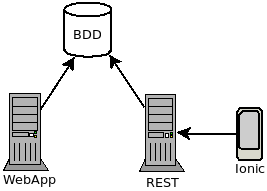
\includegraphics[width=0.45\textwidth, keepaspectratio]{res/diag_infra.png}
				\caption{La connexion à la BDD selon le projet}
			\end{figure}

			L'API ainsi que l'application web utilisent sur le Framework Spring Boot. Ces 2 applications font donc parti de 2 projets différents, "webApp" pour la partie web et "rest" pour l'api. Celles si demandant un code identique pour les Services, les Entités ainsi que les Repository, le choix a donc été fait de faire un projet commun dénommé "core" dans lequel on peut retrouver tout le code qui sera commun aux 2 autres parties, non seulement concernant les éléments cités plus haut mais également concernant les exceptions ou certains outils.

			\begin{figure}[H]
				\centering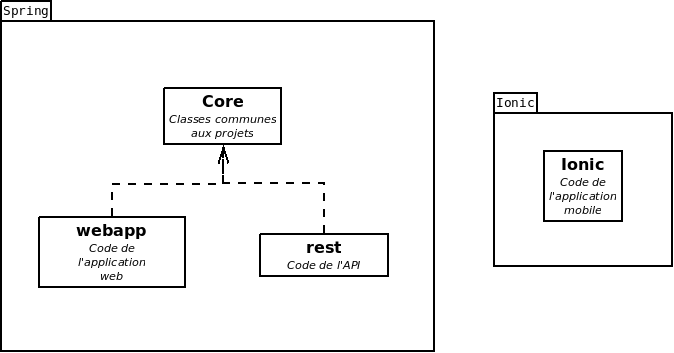
\includegraphics[width=0.75\textwidth, keepaspectratio]{res/diag_projet.png}
				\caption{Les dépendances entre les projets}
			\end{figure}

		\subsection{Configuration Gradle}

			Pour gérer correctement les différents projets basés sur Spring, leur dépendances ainsi que leur configuration nous avons donc utilisé Gradle comme mentionné plus haut. Dans le dossier "src/Spring" on retrouve le "build.gradle" qui se charge de configurer tout le projet. On peut observer la configuration suivante pour tout les projets.

			\begin{figure}[H]
				\centering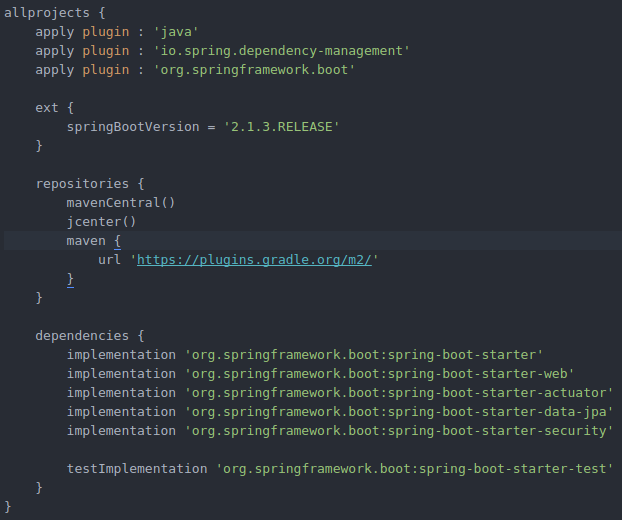
\includegraphics[width=0.75\textwidth, keepaspectratio]{res/gradle_allprojects.png}
				\caption{Configuration Gradle de tous les projets}
			\end{figure}

			On définit donc la version de Spring à utiliser, en plus des dépendences commune à chaque projet (spring-boot-starter-web, spring-boot-starter-data-jpa, ...). On va par la suite définir les dépendances uniques à chaque projet.

			\begin{figure}[H]
				\centering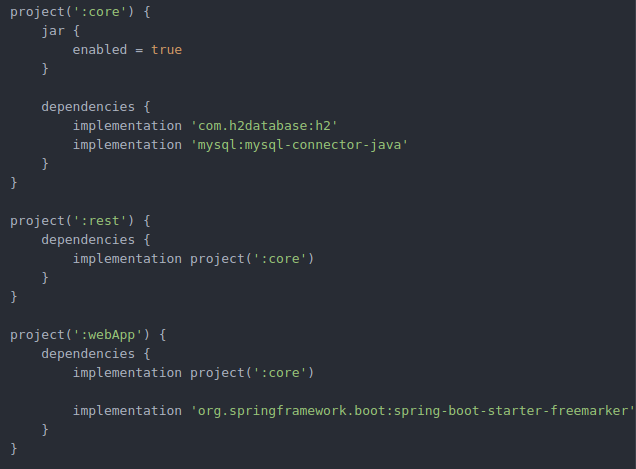
\includegraphics[width=0.75\textwidth, keepaspectratio]{res/gradle_project.png}
				\caption{Configuration Gradle individuelle des projets}
			\end{figure}

			De même, concernant le projet core, on active uniquement la compilation en jar (comme une lib) et non pas en jar bootable (comme c'est le cas lorsque l'on utilise Spring Boot).

			D'autre scripts "build.gradle" se trouvent dans chaque dossiers du projet, cependant, ceux ci ne configurent que le nom du projet à l'issue du build, la version du JDK utilisée ainsi que le package de base du projet.


	\chapter{Core}
	\section{Organisation des packages}

		L'organisation des packages se déroule comme suit :

		\begin{figure}[H]
			\centering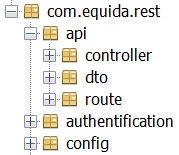
\includegraphics[width=0.33\textwidth, keepaspectratio]{res/package.png}
			\caption{Packages de Core}
		\end{figure}

		\begin{description}
			\item[authentification]{Contient toutes le classes relatives à l'authentification}
			\item[bdd]{Contient toutes les classes relative à la \bdd{}}

			\begin{description}
				\item[entity]{Contient toutes les classes Métiers}
				\item[repository]{Contient toutes les classes qui héritent de CrudRepository}
			\end{description}

			\item[converter]{Contient toutes les classes qui héritent de AttributeConverter}
			\item[exception]{Contient toutes les Exceptions}
			\item[service]{Contient toutes les classes Services}
			\item[utils]{Contient quelques classes utiles (Sha256PasswordEncoder, DateUtils, ...)}
		\end{description}

	\section{Exemple d'Entity}
		%TODO Parler de comment fonctionne nos entités

	\section{Exemple de Repository}
		%TODO Parler de comment fonctionne les répository

	\section{Exemple de Service}
		%TODO Parler de comment fonctionne nos Services

	\section{Exemple d'exception (NotFoundException)}
		Le module Core permet de fournir certaines exceptions. Actuellement elles sont au nombre de 4.

		\begin{figure}[H]
			\centering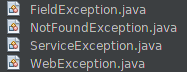
\includegraphics[width=0.30\textwidth, keepaspectratio]{res/exceptions.png}
			\caption{Les différentes exceptions}
		\end{figure}

		\begin{description}
			\item[FieldException]{Permet de signaler une erreur sur un champs d'un formulaire alors que l'information saisie est valide d'un point de vue HTML. On peut par exemple citer un sire qui n'existe pas dans la \bdd{}, un login qui existe déjà, ...}
			\item[NotFoundException]{Permet, notamment, de signaler que l'enregistrement demandé n'existe pas dans la \bdd{} ou bien que l'utilisateur n'est pas autorisé à le voir, comme c'est le cas avec un cheval qui appartient à un autre client par exemple.}
			\item[ServiceException]{Permet de signaler une erreur dans le comportement du Service. Elles sont surtout utilisés pour signaler qu'un champs requis vaut null.}
			\item[WebException]{Permet d'encapsuler une exception pour ne pas gêner l'affichage utilisateur. Lors d'un ServiceException, par exemple, l'envoie d'un WebException permet d'afficher une page d'erreur personnalisée.}
		\end{description}

		Le code des exceptions est plutot simple et court. Voici, par exemple, le code pour NotFoundException.

		\begin{figure}[H]
			\centering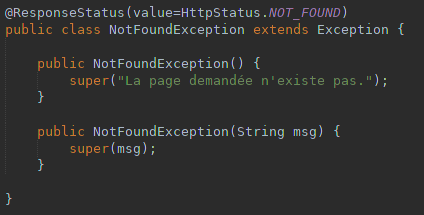
\includegraphics[width=0.75\textwidth, keepaspectratio]{res/NotFoundException.png}
			\caption{Code de NotFoundException}
		\end{figure}

		On y définit un simple message d'erreur et on change le code de réponse HTTP, grace à l'annotation ResponseStatus, pour qu'il envoie le code 404 et affiche la page adéquate.

	\section{Authentification}

		Ce package permet de gérer les différentes classes communes à l'authentification de l'utilisateur pour ce qui est du module Rest et WebApp. On y retrouve 2 classes :

		\begin{description}
		   \item[AuthentificationService]{Cette classe implémente l'interface "UserDetailsService". Elle permet pour un login donné d'aller récupérer l'utilisateur correspondant dans la \bdd{} et retourne un objet de type "AuthentificatedUser".}
		   \item[AuthentificatedUser]{Représente l'utilisateur actuellement connecté. Cette classe implémente l'interface "UserDetails". On y retient notamment la classe Compte qui est la classe métier de la table "COMPTE" dans la \bdd{}. Grace à cet attribut on pourra facilement obtenir les informations sur l'utilisateur connecté, par le biais de la méthode "Utilisateur getUtilisteur()".}
	   \end{description}

	   L'authentification sera alors géré de manière différente selon le module. Dans le cas du module WebApp il s'agira d'une connexion par le biais d'une page web tandis que pour l'api Rest on utilisera \href{https://fr.wikipedia.org/wiki/Authentification\_HTTP#M%C3%A9thode\_%C2%AB\_Basic\_%C2%BB}{Basic Authentification}.

	\section{Utils}

		\subsection{DateUtils}

			Cette classe permet de gérer certaines fonctionnalités au niveau des dates. On peut par exemple citer la méthode "boolean isBetween(Date, Date, Date)" qui permet de savoir si la dernière Date est comprise entre les 2 premières. Cette classe permet également d'aficher une date fournit en parametre au format "jour/mois/année" grâce à la méhode "String format(Date)"

		\subsection{Sha256PasswordEncoder}

			Cette classe permet de gérer le hachage des mots de passes. Elle implémente l'interface "PasswordEncoder". Celle ci fournit une méthode publique "String encode(CharSequence)" retournant en String le hachage, en sha256 dans notre cas, de la chaine de caractère fournit en paramètre. Cette classe est fournit à Spring Security afin de vérifier les informations saisies par l'utilisateur lors d'une connexion. Elle est également utilisé manuellement lors de l'enregistrement d'un nouveau client.


	\chapter{Application web}
\label{chapter:app_web}
	\section{Organisation des packages}

		\subsection{Packages}

			L'organisation des packages se présente comme suit :

			\begin{figure}[H]
				\centering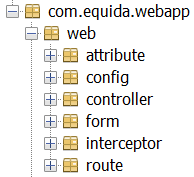
\includegraphics[width=0.33\textwidth, keepaspectratio]{res/webapp-package.png}
				\caption{Packages de WebApp}
			\end{figure}

			\begin{description}
				\item[attribute :]{Contient la classe InputOutputAttribute qui gère toutes les constantes dont on pourrait avoir besoin}
				\item[config :]{Contient les classes relatives à la configuration et la sécurité de l'application}
				\item[controller :]{Contient tous les contrôleurs qui héritent de la classe AbstractWebController}
				\item[form :]{Contient tous les formulaires qui héritent de la classe IForm}
				\item[interceptor :]{Contient la classe UserInterceptor qui hérite de HandlerInterceptorAdapter (voir \nameref{subsec:interceptor} et/ou \href{https://www.tutorialspoint.com/spring_boot/spring_boot_interceptor.htm}{là})}
				\item[route :]{Contient toutes les routes qui héritent de IRoute}
			\end{description}

		\newpage
		\subsection{Resources}

			L'organisation des ressources se présente comme suit :

			\begin{figure}[H]
				\centering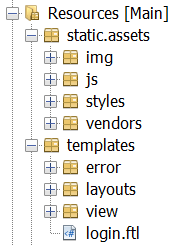
\includegraphics[width=0.23\textwidth, keepaspectratio]{res/ressources.png}
				\caption{Ressources de WebApp}
			\end{figure}

			\begin{description}
				\item[static.assets :]{Contient toutes les ressources statiques qui ne nécessitent aucune compilation}
				\begin{description}
					\item[img :]{Contient toutes les images de l'application}
					\item[js :]{Contient tous les fichiers JavaScript notamment celui pour la gestion des classements à une course d'un cheval et celui pour la page d'accueil avec son carrousel et son menu}
					\item[styles :]{Contient le fichier css de base}
					\item[vendors :]{Contient toutes les dépendances externes du projet soit : Materialize (librairie qui gère le design des vues de l'application), jQuery, Google (police de caractères)}
				\end{description}

				\item[templates :]{Contient tous les fichiers Freemarker}
				\begin{description}
					\item[error :]{Contient les fichiers ftl pour les erreurs 403, 404, 500}
					\item[layouts :]{Contient les fichiers ftl communs à toutes les pages de l'application}
					\item[view :]{Contient toutes les vues de l'applications (lister, consulter, form)}
					\item[login.ftl :]{Fichier utilisé par SpringSecurity pour la page d'authentification}
				\end{description}
			\end{description}

	\newpage
	\section{Configuration de l'application}

		\subsection{application.properties}

			L'application web possède un fichier \textit{application.properties} qui permet de configurer certaines parties de l'application.

			\begin{figure}[H]
				\centering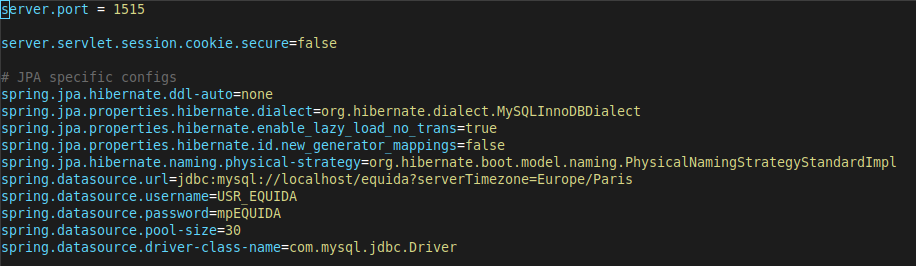
\includegraphics[width=0.85\textwidth, keepaspectratio]{res/application-properties.png}
				\caption{Configuration par application.properties}
			\end{figure}

			Ce fichier configure les informations relatives à l'application dans sa globalité, comme le port à utiliser, la configuration pour connexion avec la \bdd{} (nom utilisateur, mot de passe, ip, ...) ou encore la configuration du moteur de template, FreeMarker en l'occurence.

		\newpage
		\subsection{Configuration par le code}
			\label{subsec:webapp_configCode}

			La configuration de Spring Security est directement faite dans le code source grace à l'utilisation de l'annotation \textit{@Configuration}.

			\begin{figure}[H]
				\centering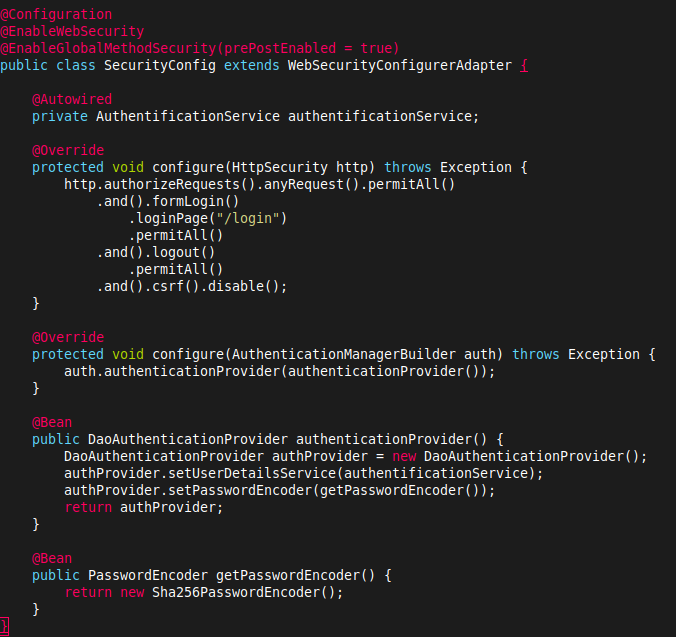
\includegraphics[width=0.75\textwidth, keepaspectratio]{res/SecurityConfig.png}
				\caption{Configuration de Spring Security}
			\end{figure}

			La méthode \textit{void configure(HttpSecurity http)} permet de configurer l'accès aux différentes pages et de changer la configuration des requêtes HTTP. Ainsi, on autorise la connexion sur toutes les pages web, d'autant plus sur login et logout. De cette manière, le jour où l'on décidera de changer cette configuration, le code pour autoriser l'accès à \textit{/logout} et \textit{/login} sera déjà présent et empêchera un potentiel oubli.

			\noindent
			Les méthodes suivantes sont relatives à l'authentification. La méthode \textit{void configure(AuthenticationManagerBuilder)} permet de changer la méthode d'authentification utilisée par Spring Security. Elle fait appel à \textit{DaoAuthenticationProvider authenticationProvider()} qui retourne le DAO à utiliser. On doit donc fournir le \textit{UserDetailsService} du module core, c'est à dire \textit{AuthentificationService} (cf : \nameref{sec:core_authentification}), et le \textit{PasswordEncoder} approprié. De ce fait on utilise donc une nouvelle instance de \textit{Sha256PasswordEncoder} (cf : \nameref{subsec:Sha256PasswordEncoder}).

	\newpage
	\section{Fichiers ressources}

		\subsection{FreeMarker}

			FreeMarker est un moteur de template basé sur Java qui est à l'origine de la génération de pages web dynamiques dans une architecture logicielle.\newline
			Comme mentionné auparavant, tous les fichiers de FreeMarker sont contenus dans le dossier \textit{/resources/templates}. Il est donc possible d'utiliser les directives propres à ce moteur de template.


			\subsubsection{Page de base}

				La page \textit{base.ftl} correspond à la page type de l'application. On y retrouve ainsi ce qui sera inclus sur toutes les pages de l'application. \newline
				Ainsi, \textit{base.ftl} contient le header de la page avec l'inclusion de la feuille de style ; sa partie body contient, elle, le contenu du fichier \textit{nav.ftl} correspondant au menu, ainsi que le footer et les fichiers de scripts nécessaires.\newline
				Les macros permettent le chargement du contenu aux endroits prévus à cet effet. Par exemple, la directive \textit{<@content/>}, présente dans le body de \textit{base.ftl}, chargera le code dans la macro \textit{content} du fichier x.ftl à cet endroit.

				\begin{figure}[H]
					\centering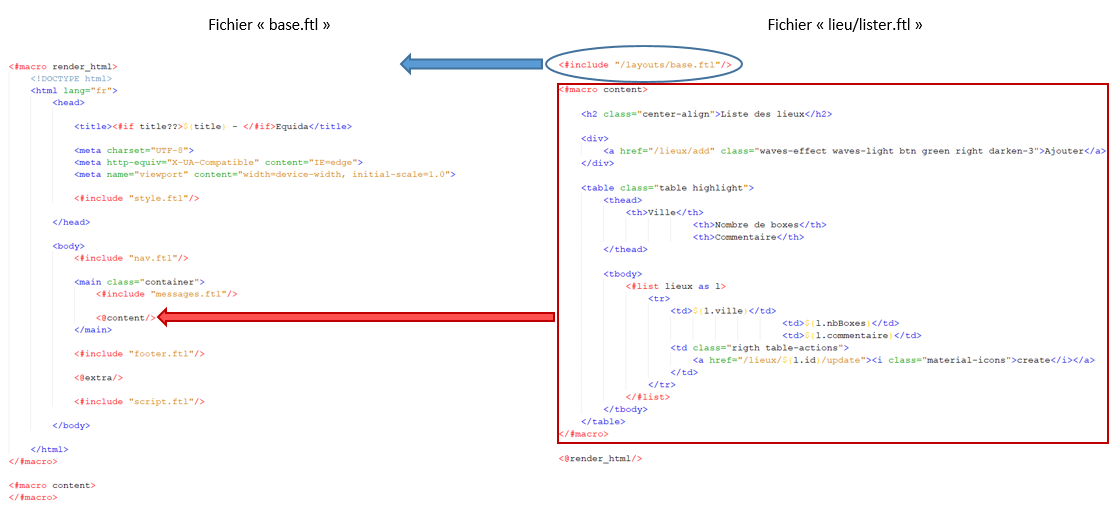
\includegraphics[width=1\textwidth, keepaspectratio]{res/fonctionnementBaseFtl.png}
					\caption{Exemple du fonctionnement de la page base.ftl avec la page lieux/lister.ftl}
				\end{figure}

				\begin{figure}[H]
					\centering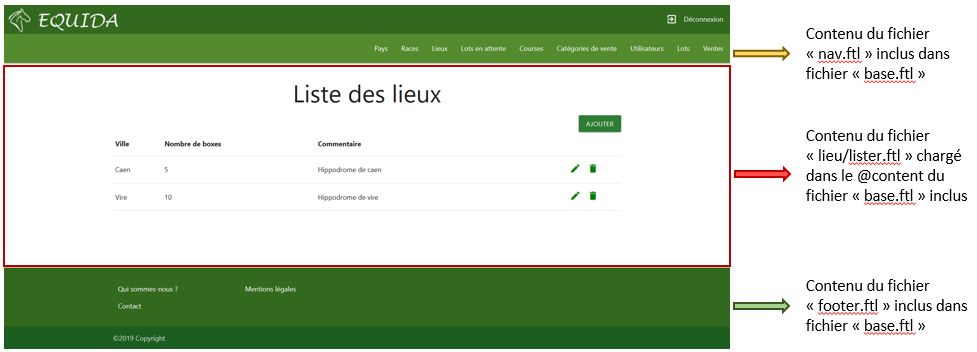
\includegraphics[width=1\textwidth, keepaspectratio]{res/exempleFonctionnementBaseLieuFtl.png}
					\caption{Rendu lors du chargement de la vue qui liste les lieux (correspondant à la page lieux/lister.ftl précédente)}
				\end{figure}

			\subsubsection{Page d'erreur}

				Les pages d'erreur sont chargées automatiquement par Spring et contiennent des messages explicites. Nous avons gérés les erreurs 403 (permissions non autorisées), 404 (page inexistante) et 500 (exception lors de l'exécution du code). Elles reprennent, elles aussi, le design de base de l'application (base.ftl).

				\begin{figure}[H]
					\centering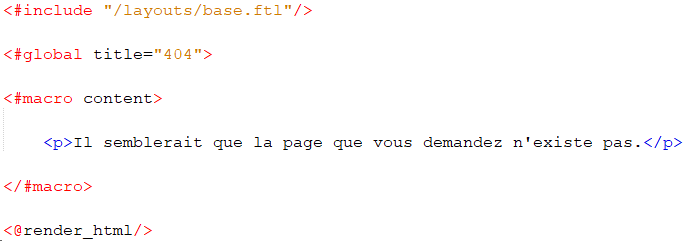
\includegraphics[width=0.75\textwidth, keepaspectratio]{res/codeErreur404.png}
					\caption{Code de l'erreur 404}
				\end{figure}

				\begin{figure}[H]
					\centering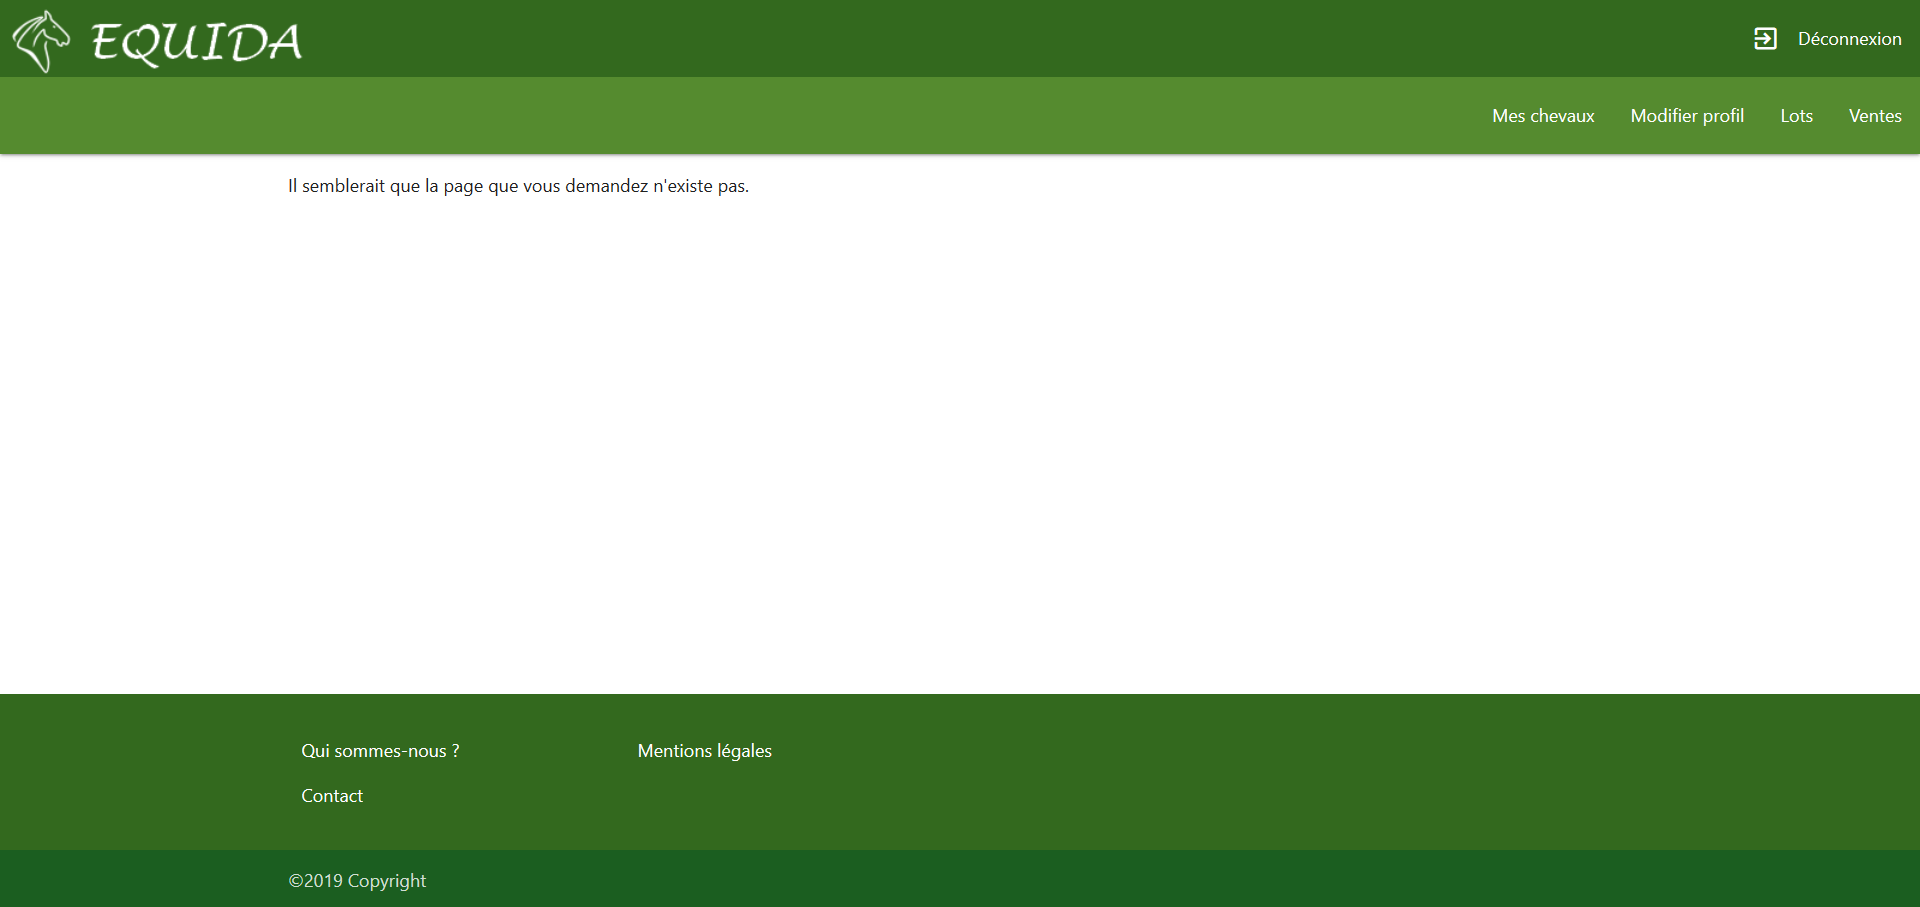
\includegraphics[width=0.85\textwidth, keepaspectratio]{res/exempleErreur404.png}
					\caption{Rendu lors d'une tentative de chargement d'une page inexistante}
				\end{figure}

			\subsubsection{Fichiers à inclure}

				Le dossier \textit{/view/include} contient les vues communes aux différentes pages. On peut les inclure en utilisant les directives \textit{<\#include />}. On retrouve par exemple le fichier \textit{lotLister} qui permet d'afficher les cartes pour les différents lots.

				\begin{figure}[H]
					\centering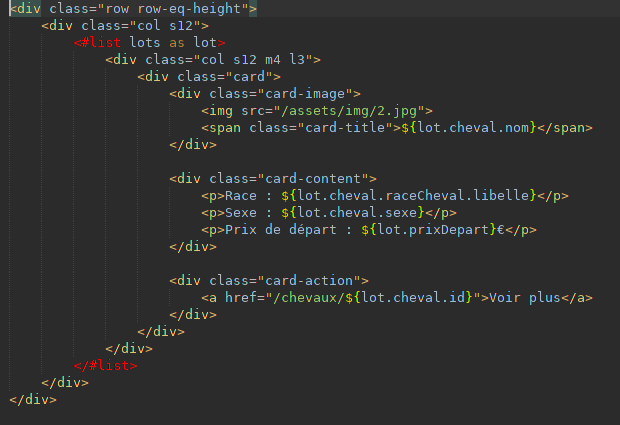
\includegraphics[width=0.75\textwidth, keepaspectratio]{res/include-lotLister.png}
					\caption{Extrait de code du fichier lotLister}
				\end{figure}

				Le code reste celui de n'importe quelle autre vue et ne comporte aucune spécificité.

			\subsubsection{Exemple de page web}

				Ainsi, avec tous les éléments cités précédemment, on peut créer des vues telles que celle ci :

				\begin{figure}[H]
					\centering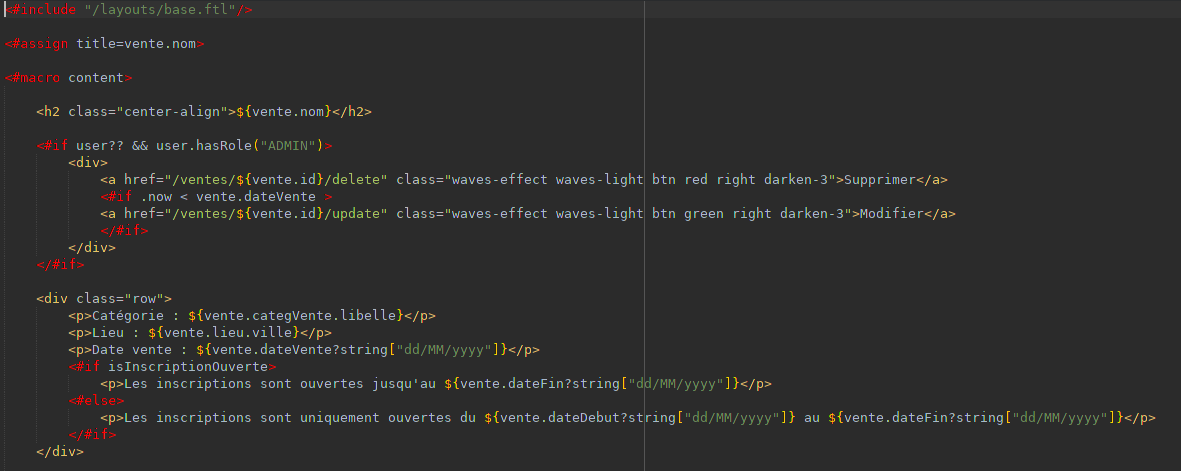
\includegraphics[width=0.85\textwidth, keepaspectratio]{res/view-venteConsulter.png}
					\caption{Code de la vue pour la consultation d'une vente}
				\end{figure}
				On retrouve donc, l'include de \textit{/layouts/base.ftl} pour reprendre le template de base, un changement de valeur concernant le titre, l'utilisation de la macro content, ...

	\section{Gestion de l'authentification}

		\subsection{Gestion template et controller}

			Un contrôleur existe afin de gérer l'affichage d'un template FreeMarker concernant la page de connexion à l'application. Ce contrôleur se charge uniquement de l'affichage de l'information. En effet, le traitement des identifiants est fait par Spring Security (comme mentionné dans \nameref{subsec:webapp_configCode}).

		\subsection{Interceptor}
			\label{subsec:interceptor}

			Afin de faciliter la gestion de l'utilisateur actuellement connecté dans la vue ou les contrôleurs, une classe \textit{UserInterceptor} permet de fournir automatiquement l'instance de \textit{AuthentificatedUser} à la vue ou au contrôleur.

			\begin{figure}[H]
				\centering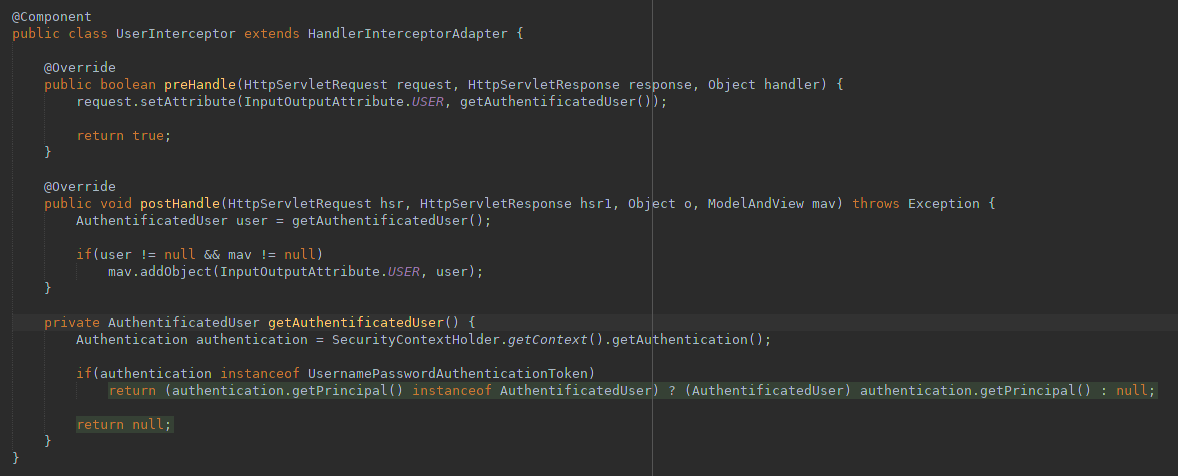
\includegraphics[width=0.85\textwidth, keepaspectratio]{res/UserInterceptor.png}
				\caption{Code de UserInterceptor}
			\end{figure}

			\noindent
			On peut alors avoir accès à la variable \textit{user} dans la vue comme n'importe quelle variable fournie par le contrôleur ou dans le contrôleur en utilisant le paramètre suivant dans une méthode d'un controleur \textit{@RequestAttribute(name = InputOutputAttribute.USER, required = false) AuthentificatedUser user}.

	\section{Exemple Route}

		L'interface \textit{IRoute} décrit les méthodes qui doivent être implémentées par les classes filles.\newline
		Ainsi chaque fichier route contiendra une méthode \textit{getUri()}, une méthode \textit{getView()} et \textit{getTitle()} qui retourneront respectivement l'URL, la vue et le titre à utiliser dans la page concernée (pour la route correspondante).

		\noindent
		Par exemple, pour \textit{PaysRoute}, qui est donc la route principale selon notre nomenclature, l'URL correspond à \textit{/pays}, c'est à cette url là, qu'on chargera la vue \textit{pays/lister} avec le titre "Les pays".

		\begin{figure}[H]
			\centering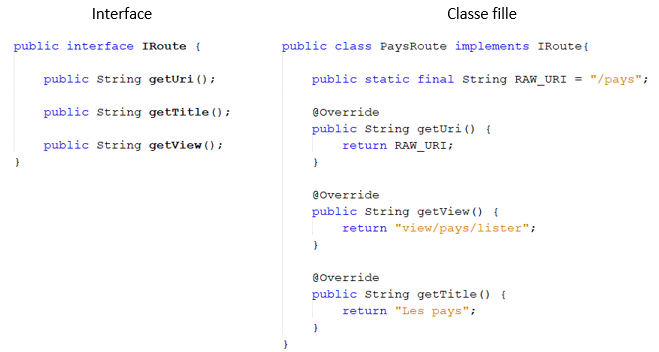
\includegraphics[width=0.75\textwidth, keepaspectratio]{res/paysRoute.png}
			\caption{Code de l'interface et utilisation par la classe fille PaysRoute}
		\end{figure}

		\begin{figure}[H]
			\centering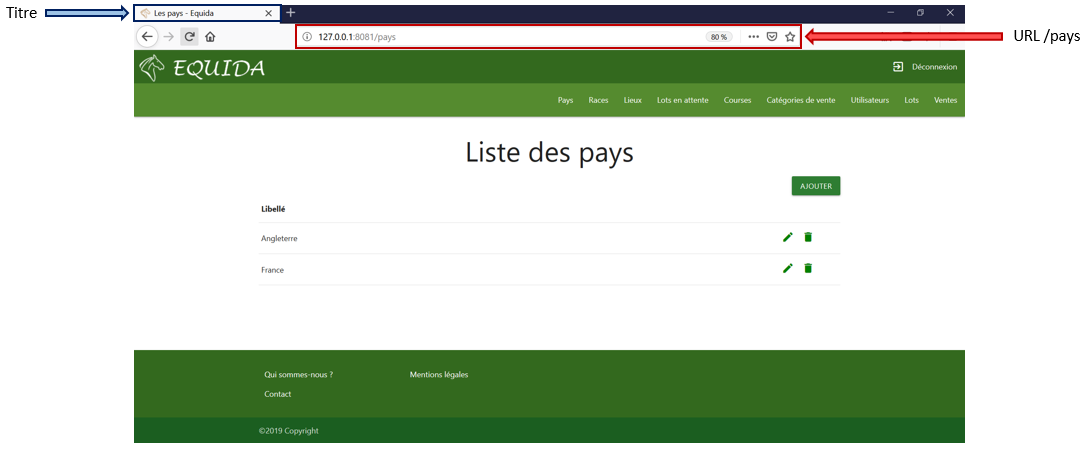
\includegraphics[width=0.85\textwidth, keepaspectratio]{res/renduPaysRoute.png}
			\caption{Rendu obtenu avec la vue pays/lister}
		\end{figure}

	\section{Exemple Form}

		La classe mère \textit{IForm} est une classe abstraite qui utilise la générécité ce qui nous permettra d'adapter les méthodes en fonction de l'entité x pour laquelle le formulaire est fait. L'héritage nous permet donc d'utiliser les variables et méthodes déclarées dans le formulaire neutre xForm.\newline
		Par exemple, prenons l'entité \textit{Lieu}. On crée le formulaire "neutre" \textit{LieuxForm} qui héritera de \textit{IForm} et qui permettra de définir les éléments communs aux formulaire d'ajout et de modification.\newline
		On fera donc hériter de ce formulaire "neutre" \textit{LieuxAddForm} et \textit{LieuxUpdateForm} et on passera, dans un premier cas, le la variable \textit{isCreation} à true et dans le second, à false.

		\begin{figure}[H]
			\centering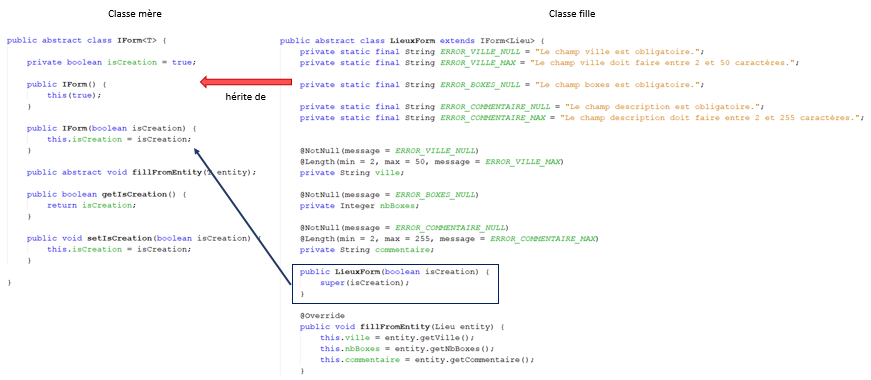
\includegraphics[width=1\textwidth, keepaspectratio]{res/IForm.png}
			\caption{Exemple implémentation interface IForm avec LieuxForm}
		\end{figure}

		\begin{figure}[H]
			\centering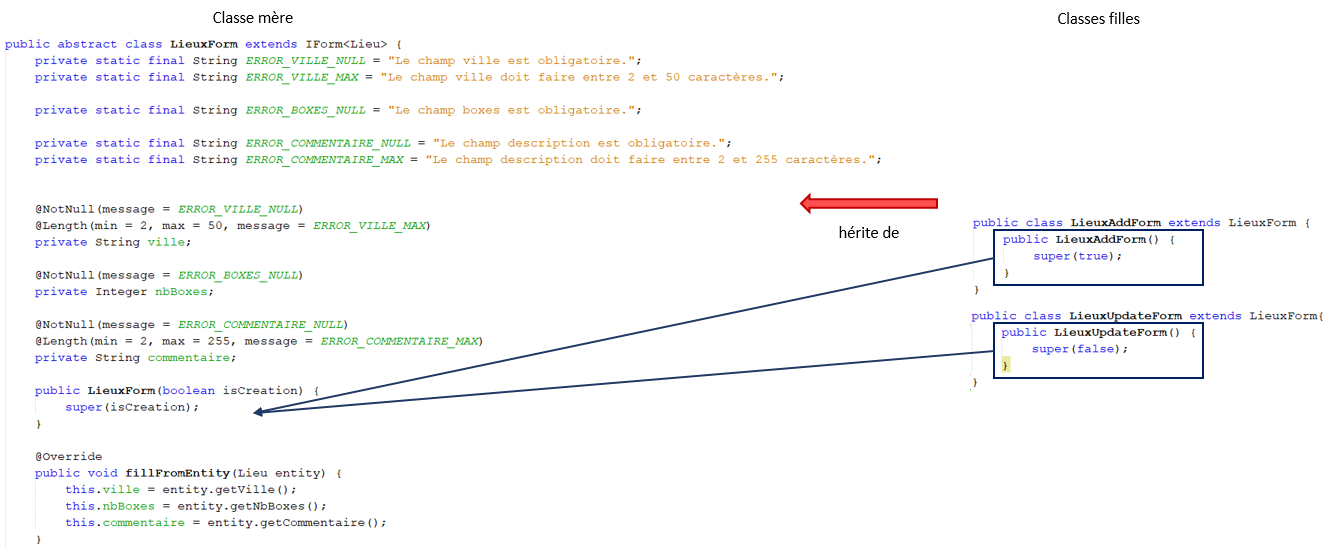
\includegraphics[width=1\textwidth, keepaspectratio]{res/formClassFilles.png}
			\caption{Exemple avec LieuxUpdateForm et LieuxAddForm}
		\end{figure}

	\newpage
	\section{Classe InputOutputAttribute}

		Cette classe permet la définition de constantes qui seront utilisées au travers de l'application.

		\begin{figure}[H]
			\centering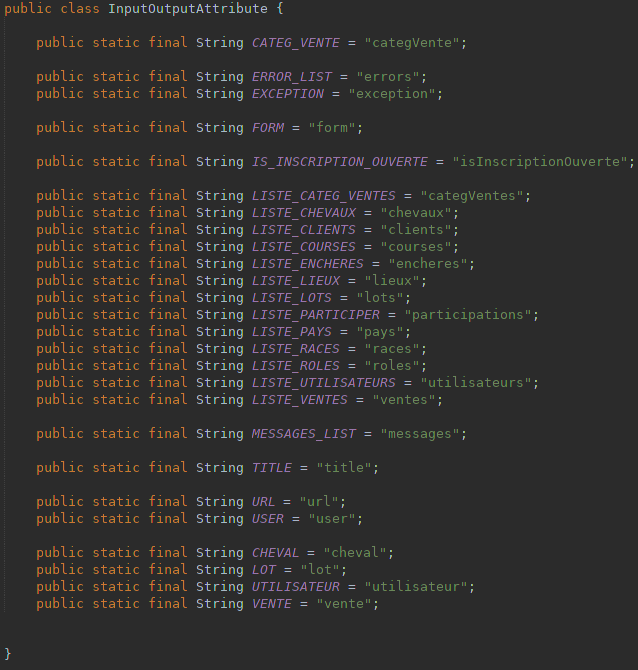
\includegraphics[width=0.75\textwidth, keepaspectratio]{res/InputOutputAttribute.png}
			\caption{Code de InputOutputAttribute}
		\end{figure}

		Ces constantes permettent de garder une unité dans la définition des noms et d'éviter d'éventuelles erreurs d'écriture. Ainsi, lorsque l'on doit fournir une clé de type String on pourra utiliser une des constantes de la classe. Elles sont donc très utilisées pour transmettre les informations du contrôleur vers la vue.

		\begin{figure}[H]
			\centering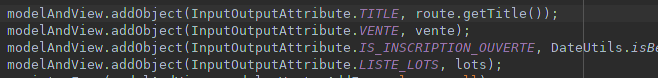
\includegraphics[width=0.75\textwidth, keepaspectratio]{res/InputOutputAttribute-controller.png}
			\caption{Exemple d'utilisation de InputOutputAttribute}
		\end{figure}

	\newpage
	\section{Les Contrôleurs}

		\subsection{AbstractWebController}

			Cette classe est la classe mère de tous les contrôleurs. On y définit certaines méthodes, par exemple, la possibilité d'ajouter des messages d'erreurs, qui seront transférées à la vue.

			\begin{figure}[H]
				\centering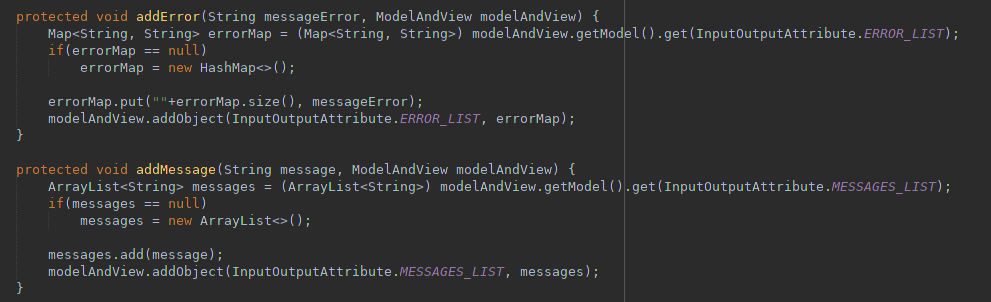
\includegraphics[width=0.85\textwidth, keepaspectratio]{res/AbstractWebController-messages.png}
				\caption{Méthodes pour la gestion des messages}
			\end{figure}

			\noindent
			On y implémente aussi la gestion des exceptions, dans lesquelles, on passe les variables nécessaires au bon affichage de la vue.

			\begin{figure}[H]
				\centering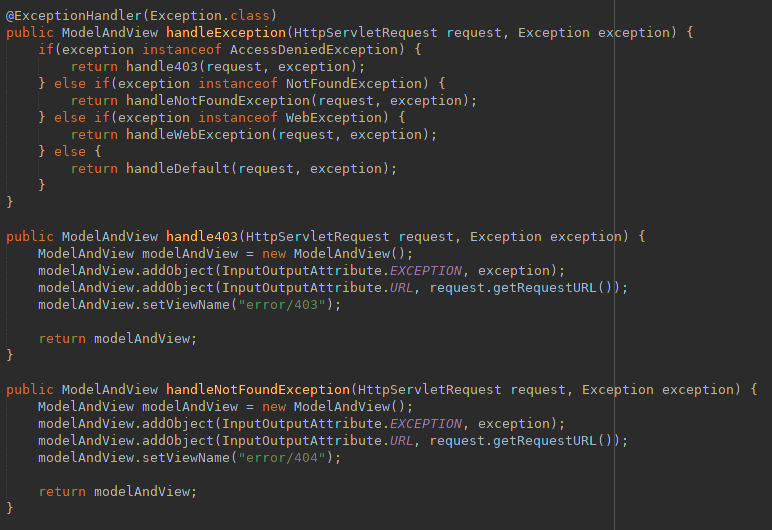
\includegraphics[width=0.75\textwidth, keepaspectratio]{res/AbstractWebController-exception.png}
				\caption{Méthodes pour la gestion des exceptions}
			\end{figure}

			\newpage
			\noindent
			Elle comprend, en plus, 2 méthodes qui permettent de simplifier le code de gestion des formulaires, l'une afin de les créer et de les compléter si besoin, l'autre afin de faciliter la gestion des erreurs sur ceux-ci.

			\begin{figure}[H]
				\centering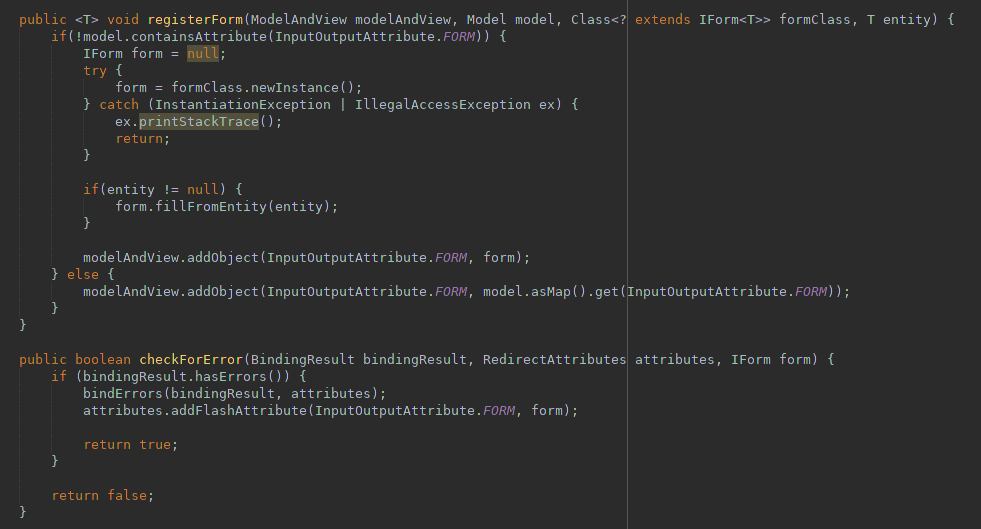
\includegraphics[width=0.80\textwidth, keepaspectratio]{res/AbstractWebController-form.png}
				\caption{Méthodes pour la gestion des formulaires}
			\end{figure}

		\subsection{Exemple Controller}

		Les différents contrôleurs créés pour les entités x héritent tous de la classe AbstractWebController. \newline
		Les contrôleurs contiennent différentes méthodes associées aux méthodes GET, POST, PATCH et DELETE ainsi qu'a une route. Enfin, elles utilisent les services pour intéragir avec la \bdd{}. On y définit aussi les différentes autorisations avec l'annotation @PreAuthorize afin de savoir qui peut accéder à la page, et donc, executer la méthode.

		\noindent
		Par exemple, dans \textit{EncheresController}, la méthode \textit{addGet} n'est possible que pour un utilisateur ayant le role 'ADMIN', elle est reliée à l'URL \textit{EncheresAddRoute.RAW\_URI} (URL stockée dans la variable constante RAW\_URI de la classe \textit{EncheresAddRoute}). Elle permet de récupérer les différentes variables nécessaires à l'affichage de la page, comme le formulaire d'ajout d'une enchère par exemple.

		\begin{figure}[H]
			\centering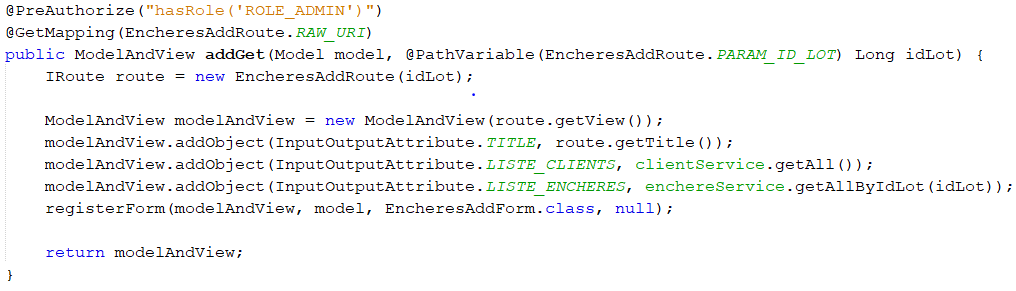
\includegraphics[width=0.95\textwidth, keepaspectratio]{res/enchereController.png}
			\caption{Exemple d'un contrôleur}
		\end{figure}


	\chapter{Application mobile}
	\section{API REST}
	\section{Organisation des packages}

	\section{Ionic}
	\section{Organisation des packages}


	\chapter{Ressources}

\noindent
Github du projet : \url{https://github.com/justine-martin-study/Equida}\\
Trello : \url{https://trello.com/b/jrKixhpu/equida-spring}


\end{document}

% Aide pour la prise enmain de Latex.
% Les lignes qui commencent par "%" sont des commentaires.

% =========================

% Structurer un document

% Dans l'ordre on retrouve les éléments suivants :

% \part{part name}
% \chapter{chapter name}
% \section{section name}
% \subsection{subsection name}
% \subsubsection{subsubsection name}

% =========================

% Afficher une image

%	\begin{figure}[H]
%		\centering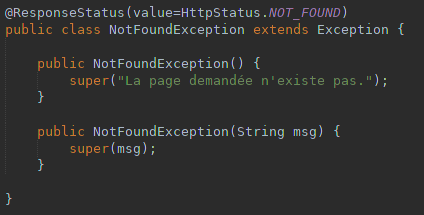
\includegraphics[width=0.75\textwidth, keepaspectratio]{res/NotFoundException.png}
%		\caption{Code de NotFoundException}
%	\end{figure}

% caption permet d'afficher une légende
% width permet de définir la taille en largeur de l'image par rapport à la taille de la feuille (ici 75%)
% res/NotFoundException.png -> Nom de l'image

% =========================

% Faire une liste à points

%	Blablabla, ainsi on peut citer :
%	\begin{itemize}
%		\item{signaler une erreur}
%		\item{mieux gérer les ...}
%	\end{itemize}

% =========================

% Faire une liste descriptive

%	Blablabla, on a donc les éléments suivants :
%	\begin{description}
%		\item[Service]{Fait l'intermédiaire entre ...}
%		\item[Repository]{Permet de faire ...}
%	\end{description}
